%%%%%%%%%%%%%%%%%%%%%%%%%%%%%%%%%%%%%%%%%
% Beamer Presentation
% LaTeX Template
% Version 1.0 (10/11/12)
%
% This template has been downloaded from:
% http://www.LaTeXTemplates.com
%
% License:
% CC BY-NC-SA 3.0 (http://creativecommons.org/licenses/by-nc-sa/3.0/)
%
% Modified by Jeremie Gillet in November 2015 to make an OIST Skill Pill template
%
%%%%%%%%%%%%%%%%%%%%%%%%%%%%%%%%%%%%%%%%%

%----------------------------------------------------------------------------------------
%	PACKAGES AND THEMES
%----------------------------------------------------------------------------------------

\documentclass{beamer}

\mode<presentation> {

\usetheme{}

\definecolor{OISTcolor}{rgb}{0.65,0.16,0.16}
\usecolortheme[named=OISTcolor]{structure}

%\setbeamertemplate{footline} % To remove the footer line in all slides uncomment this line
\setbeamertemplate{footline}[frame number] % To replace the footer line in all slides with a simple slide count uncomment this line

\setbeamertemplate{navigation symbols}{} % To remove the navigation symbols from the bottom of all slides uncomment this line

\setbeamertemplate{footline}{
  \hfill%
  \usebeamercolor[fg]{page number in head/foot}%
  \usebeamerfont{page number in head/foot}%
  \setbeamertemplate{page number in head/foot}[framenumber]%
  \usebeamertemplate*{page number in head/foot}\kern1em\vskip2pt%
}

}

\usepackage{graphicx} % Allows including images
\usepackage{booktabs} % Allows the use of \toprule, \midrule and \bottomrule in tables
\usepackage{textpos} % Use for positioning the Skill Pill logo
\usepackage{fancyvrb}
\usepackage{tikz}
\usepackage{hyperref}
\usepackage{listings}
\usepackage{movie15}
%\usepackage{multimedia}
\usepackage{xcolor}
\usepackage{braket}

\definecolor{dkgreen}{rgb}{0,0.6,0}
\definecolor{gray}{rgb}{0.5,0.5,0.5}
\definecolor{mauve}{rgb}{0.58,0,0.82}
\setbeamertemplate{frametitle}[default][center]

\lstset{frame=tb,
  language=python,
  aboveskip=3mm,
  belowskip=3mm,
  showstringspaces=false,
  columns=flexible,
  basicstyle={\small\ttfamily},
  numbers=none,
  numberstyle=\tiny\color{gray},
  keywordstyle=\color{blue},
  commentstyle=\color{dkgreen},
  stringstyle=\color{mauve},
  breaklines=true,
  breakatwhitespace=true,
  tabsize=3
}

%----------------------------------------------------------------------------------------
%	TITLE PAGE
%----------------------------------------------------------------------------------------

\title[OIST Mini-course]{GPU computing with Julia} % The short title appears at the bottom of every slide, the full title is only on the title page

\author{James Schloss} % Your name
\institute[OIST] % Your institution as it will appear on the bottom of every slide, may be shorthand to save space

\date{August 13, 2021} % Date, can be changed to a custom date

\begin{document}

\setbeamertemplate{background}{
\includegraphics[width=\paperwidth]{OISTBG.png}} % Adding the background logo

\begin{frame}
\vspace*{1.4cm}
\titlepage % Print the title page as the first slide
\end{frame}


\setbeamertemplate{background}{} % No background logo after title frame

\addtobeamertemplate{frametitle}{}{% Adding the Skill Pill logo on the title screen after title frame
\begin{textblock*}{100mm}(.92\textwidth,-0.75cm)

\includegraphics[height=1cm]{OIST}
\end{textblock*}}

\begin{frame}
\frametitle{Overview}

\begin{itemize}
\pause
\item What is a GPU?
\pause
\item What is Julia?
\pause
\item What is CUDA?
\pause
\item What is Kernel Abstractions?
\pause
\item What is a more complicated example?
\pause
\item What is the meaning of life?
\end{itemize}
\end{frame}

\begin{frame}
\frametitle{What is a GPU?}
\pause
\begin{center}
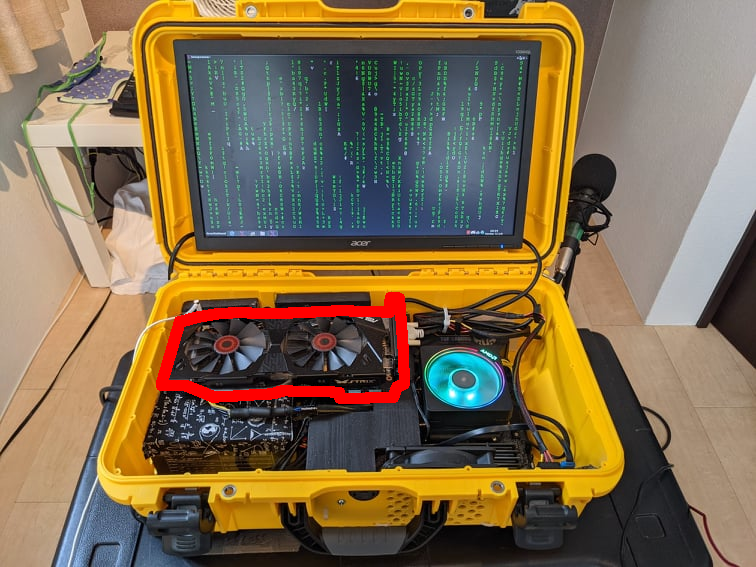
\includegraphics[width=0.75\textwidth]{wiag.png}
\end{center}
\center \Huge This thing
\end{frame}

\begin{frame}
\frametitle{Yeah, but what does it do?}
\pause
\begin{center}
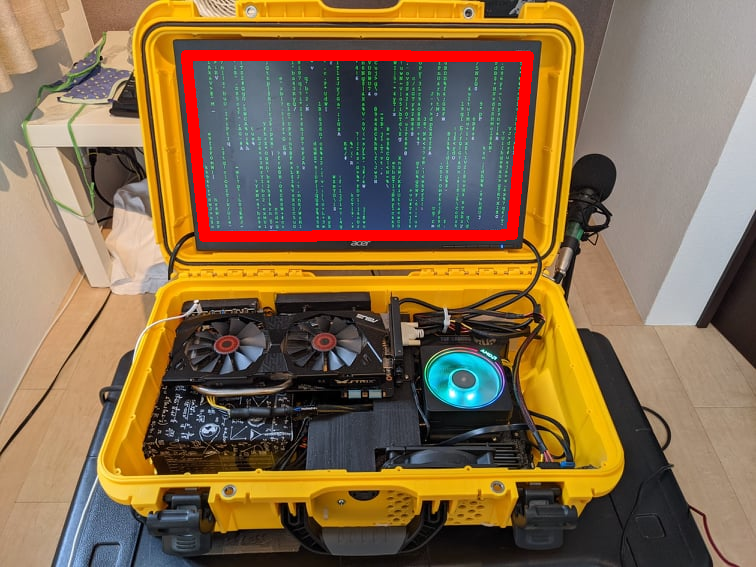
\includegraphics[width=0.75\textwidth]{ybwdid.png}
\end{center}
\center \Huge Graphics

\pause
\center \small (In parallel, though)
\end{frame}

\begin{frame}
\frametitle{Ok, but why should I care?}
\pause

\center \Huge Dunno, dawg. You are the one that decided to attend this mini-course
\end{frame}

\begin{frame}
\frametitle{Ok, but why should I care?}

\center \Huge If used correctly, GPUs can be much faster for certain tasks

\pause

\center \small (But they can also be way slower for other tasks)
\end{frame}

\begin{frame}
\frametitle{Right. How do they work?}
\begin{columns}
\column{0.5\textwidth}
\begin{itemize}
\onslide<2->
\item The Grid is split into Blocks
\item Blocks are split into Threads
\onslide<3->
\item Threads have local memory
\item Everything has global memory
\onslide<4->
\item Shared mem is faster than global memory, but a pain to use
\end{itemize}
\column{0.5\textwidth}
\begin{center}

\onslide<2->
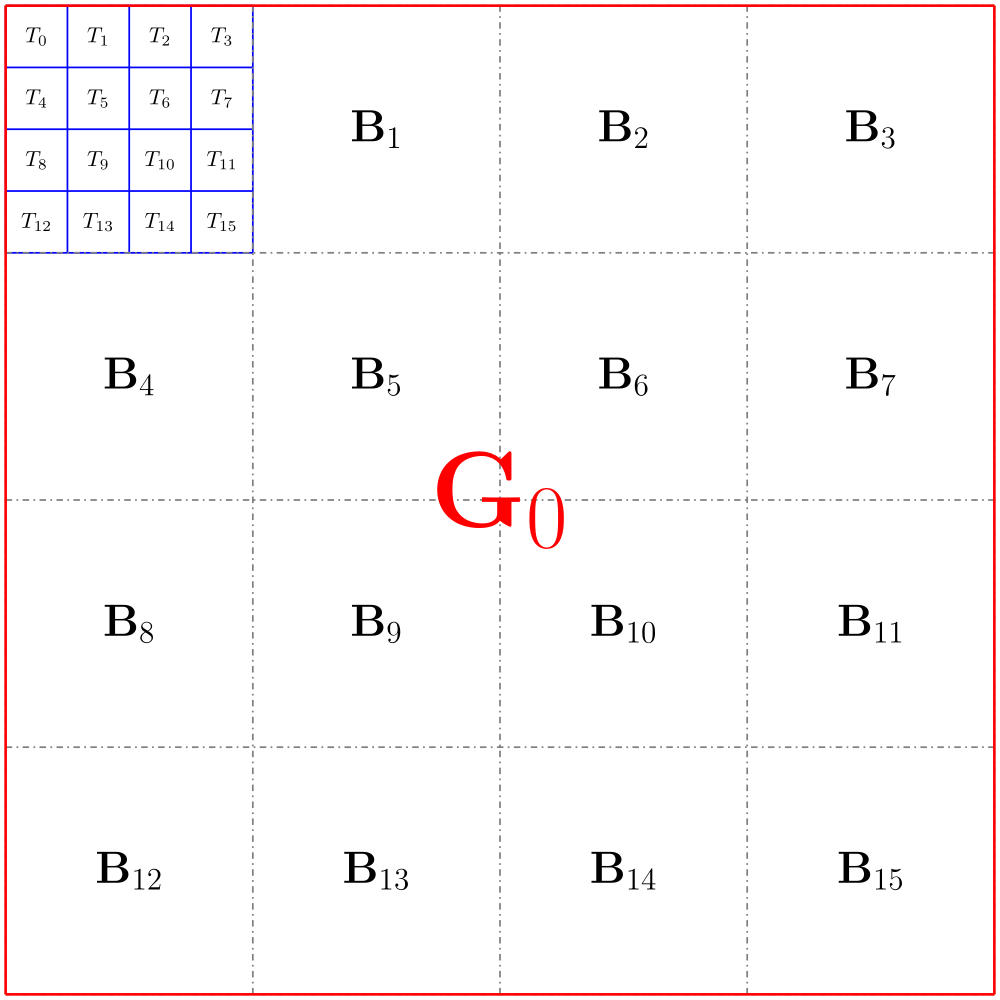
\includegraphics[width=\textwidth]{gputhreads.png}
\end{center}
\end{columns}
\end{frame}

\begin{frame}
\frametitle{What are they bad at?}
\center Ah, like everything

\begin{columns}
\column{0.5\textwidth}
\begin{itemize}
\onslide<2->
\item Iterative things are bad because threads are weak
\onslide<3->
\item Really big problems ($> 32$ GB) are bad because we have limited memory
\onslide<4->
\item Recursive things are bad because threads are weak and we have limited memory
\onslide<5->
\item Good luck getting data off the GPU and onto your SSD with any reasonable speed
\onslide<6->
\item Please don't do multi-GPU. Just... Please.
\end{itemize}
\column{0.5\textwidth}
\begin{center}

\onslide<2->
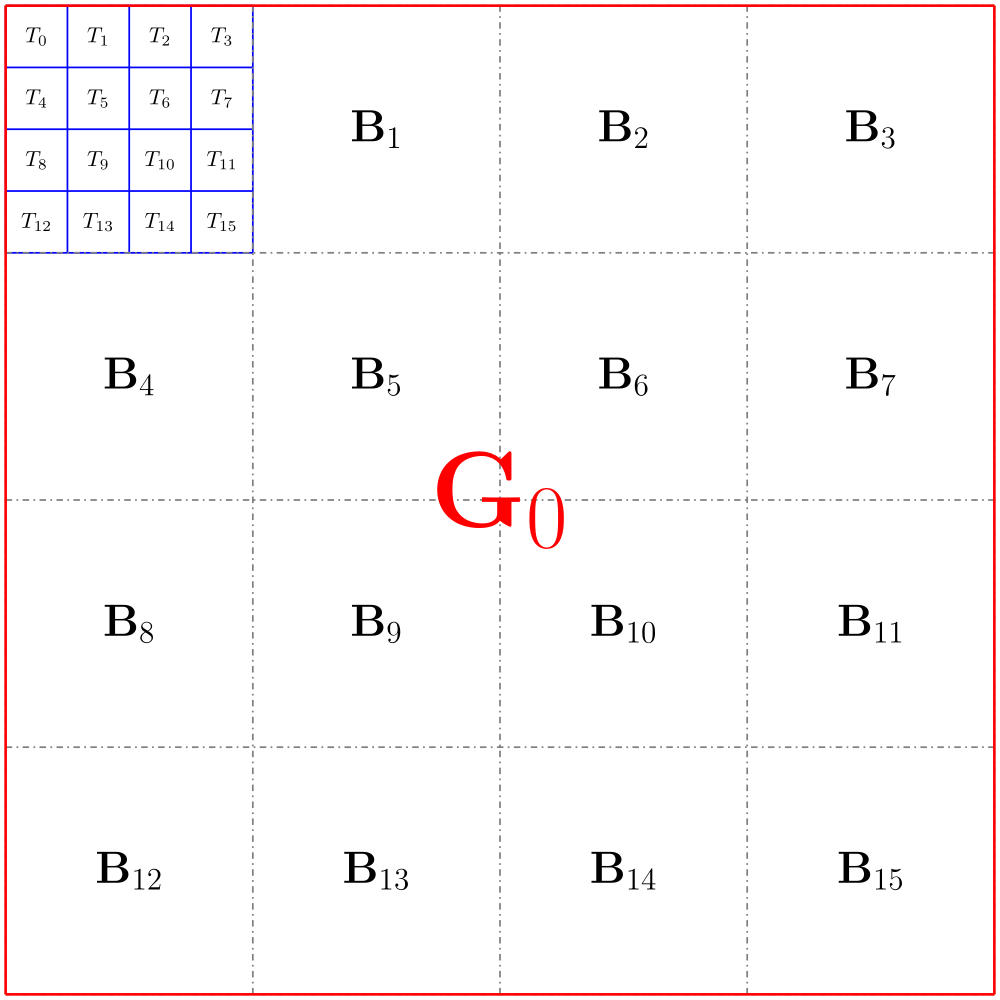
\includegraphics[width=\textwidth]{gputhreads.png}
\end{center}
\end{columns}
\end{frame}

\begin{frame}
\frametitle{So, uh...}

But, I mean, they can do matrix operations quickly, so there's that.
\end{frame}

\begin{frame}
\frametitle{but...}

\begin{centering}
Pop-quiz: 
What's the slowest part of any $n$-dimensional FFT operation?
\end{centering}

\pause
\center The transpose
\end{frame}

\begin{frame}
\frametitle{What is Julia?}

\center Live demo (hopefully)

\end{frame}

\begin{frame}
\frametitle{What is CUDA}

\center Again, live demo
\end{frame}

\begin{frame}
\frametitle{What is CUDA.jl}

\center We are doing it live!
\end{frame}

\begin{frame}
\frametitle{What is Kernel Abstractions}

\center Why did you even make these slides?
\end{frame}

\end{document}
